\documentclass[journal,10pt,twocolumn]{article}
\usepackage{graphicx, float}
\usepackage[margin=0.5in]{geometry}
\usepackage{amsmath, bm}
\usepackage{array}
\usepackage{booktabs}
\providecommand{\norm}[1]{\lVert#1\rVert}
\let\vec\mathbf
\newcommand{\myvec}[1]{\ensuremath{\begin{pmatrix}#1\end{pmatrix}}}
\newcommand{\mydet}[1]{\ensuremath{\begin{vmatrix}#1\end{vmatrix}}}

\title{\textbf{CONIC}}
\author{VEMULAPALLI BAVYA SRI}
\date{October 2022}

\begin{document}

\maketitle
\paragraph{\textit{Problem Statement} - Find the area of the region bounded by the ellipse 
$\frac{x^2}{16} + \frac{y^2}{9} = 1$}
  
\section{Solution}

    Given, 
    
    \begin{equation}
        \frac{x^2}{16} + \frac{y^2}{9} = 1
    \end{equation}
    
    The standard equation of the conics is given as
    \begin{equation}
        \Vec{x^\top}\Vec{V}\Vec{x} + 2\Vec{u^\top}\Vec{x} + f = 0
    \end{equation}
    
    By Comparing equations (1) and (2) we get,
    \begin{equation}
        \Vec{V} = \myvec{9 & 0 \\ 0 & 16} , \Vec{u} = \myvec{0 \\ 0} , f = -144
    \end{equation}
    
    Comparing eq (1) with the general form of ellipse,
    \begin{equation}
        a = 4 , b = 3
    \end{equation}
    
    The Vertices of the ellipse are given as
    \begin{equation}
        \Vec{A} = \myvec{4 \\ 0}
    \end{equation}
    
    Area bounded by the ellipse is given by,
    \begin{equation}
    Area = 4 \times area of \boldsymbol{OAB}
    \end{equation}
    
    \begin{equation}
        = 4 \times \int_{0}^{a} f(x) \ dx 
    \end{equation}
    
    \begin{equation}
        = 4 \times \int_{0}^{4} \frac{3}{4} \sqrt{16 - x^2} \ dx 
    \end{equation}
    
    By solving eq (8) we get the required area as
    \begin{equation}
        \boxed{Area = 12\pi \ units}
    \end{equation}
    
\section{Construction}

\begin{table}[h]
	\centering
\setlength\extrarowheight{2pt}
	\begin{tabular}{|c|c|c|}
		\hline
		\textbf{Symbol} & \textbf{Value} & \textbf{Description} \\
		\hline
		O & (0,0) & Origin\\
		\hline
		A & (4,0) & point A\\
		\hline
		B & (0,3) & point B\\
		\hline
		C & (-4,0) & point C\\
		\hline
		D & (0,-3) & point D\\
		\hline
	\end{tabular}
\end{table}

\begin{figure}[H]
    \centering
    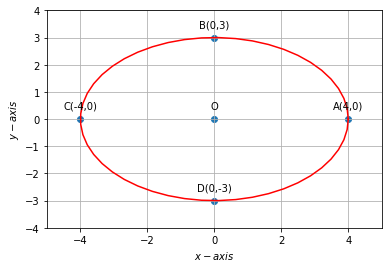
\includegraphics[scale=0.5]{conic.jpg}
    \caption{Bisector}
    \label{fig:Bisector}
\end{figure}

    The above construction is realized by executing the following code.
    
\begin{table}[H]
\begin{tabular}{|l|c|c|c|c|c|c|c|c}\hline\textbf{https://raw.githubusercontent.com}\\
    \textbf{/BavyaVemulapalli/FWC-IITH/main} \\
    \textbf{/Conic/Code/conic.py} \\ \hline
\end{tabular}
\end{table}

\section{Conclusion}

    Hence, the area of the region bounded by the given ellipse was found.

\end{document}